% TikZ/PGFPlots figure - Temperature vs Time
% This file is included directly in the LaTeX document
% To compile standalone: pdflatex -jobname=sample_plot "\documentclass{standalone}\usepackage{pgfplots}\begin{document}% TikZ/PGFPlots figure - Temperature vs Time
% This file is included directly in the LaTeX document
% To compile standalone: pdflatex -jobname=sample_plot "\documentclass{standalone}\usepackage{pgfplots}\begin{document}% TikZ/PGFPlots figure - Temperature vs Time
% This file is included directly in the LaTeX document
% To compile standalone: pdflatex -jobname=sample_plot "\documentclass{standalone}\usepackage{pgfplots}\begin{document}% TikZ/PGFPlots figure - Temperature vs Time
% This file is included directly in the LaTeX document
% To compile standalone: pdflatex -jobname=sample_plot "\documentclass{standalone}\usepackage{pgfplots}\begin{document}\input{sample_plot.tex}\end{document}"

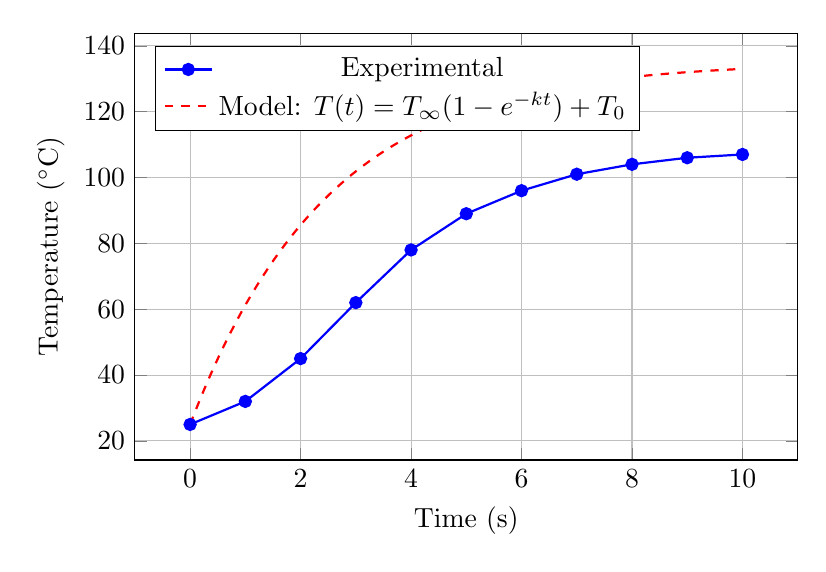
\begin{tikzpicture}
    \begin{axis}[
        width=10cm,
        height=7cm,
        xlabel={Time (s)},
        ylabel={Temperature ($^\circ$C)},
        grid=major,
        legend pos=north west,
        ylabel near ticks,
        xlabel near ticks
    ]
    
    % Sample data - exponential heating curve
    \addplot[blue, thick, mark=*, mark size=2pt] coordinates {
        (0, 25) (1, 32) (2, 45) (3, 62) (4, 78) 
        (5, 89) (6, 96) (7, 101) (8, 104) (9, 106) (10, 107)
    };
    \addlegendentry{Experimental}
    
    % Theoretical curve
    \addplot[red, thick, dashed, domain=0:10, samples=100] 
        {110*(1-exp(-0.4*x)) + 25};
    \addlegendentry{Model: $T(t) = T_{\infty}(1-e^{-kt}) + T_0$}
    
    \end{axis}
\end{tikzpicture}
\end{document}"

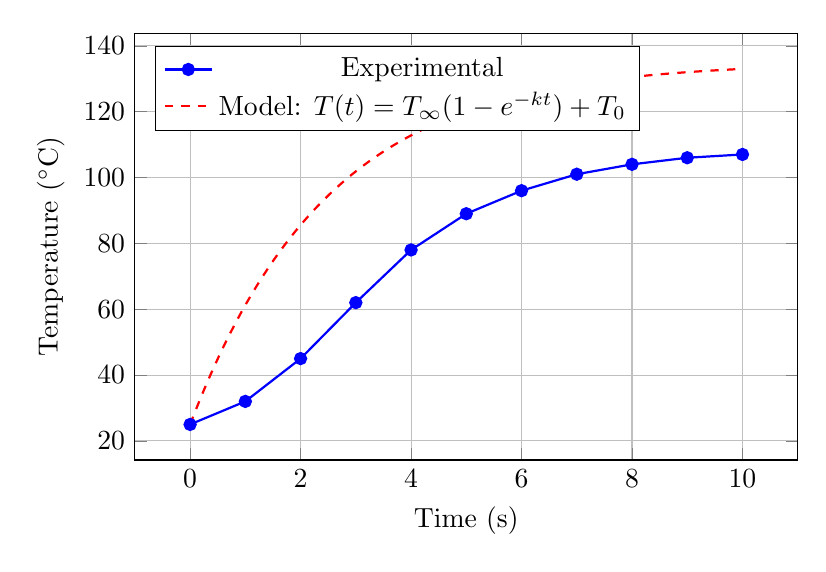
\begin{tikzpicture}
    \begin{axis}[
        width=10cm,
        height=7cm,
        xlabel={Time (s)},
        ylabel={Temperature ($^\circ$C)},
        grid=major,
        legend pos=north west,
        ylabel near ticks,
        xlabel near ticks
    ]
    
    % Sample data - exponential heating curve
    \addplot[blue, thick, mark=*, mark size=2pt] coordinates {
        (0, 25) (1, 32) (2, 45) (3, 62) (4, 78) 
        (5, 89) (6, 96) (7, 101) (8, 104) (9, 106) (10, 107)
    };
    \addlegendentry{Experimental}
    
    % Theoretical curve
    \addplot[red, thick, dashed, domain=0:10, samples=100] 
        {110*(1-exp(-0.4*x)) + 25};
    \addlegendentry{Model: $T(t) = T_{\infty}(1-e^{-kt}) + T_0$}
    
    \end{axis}
\end{tikzpicture}
\end{document}"

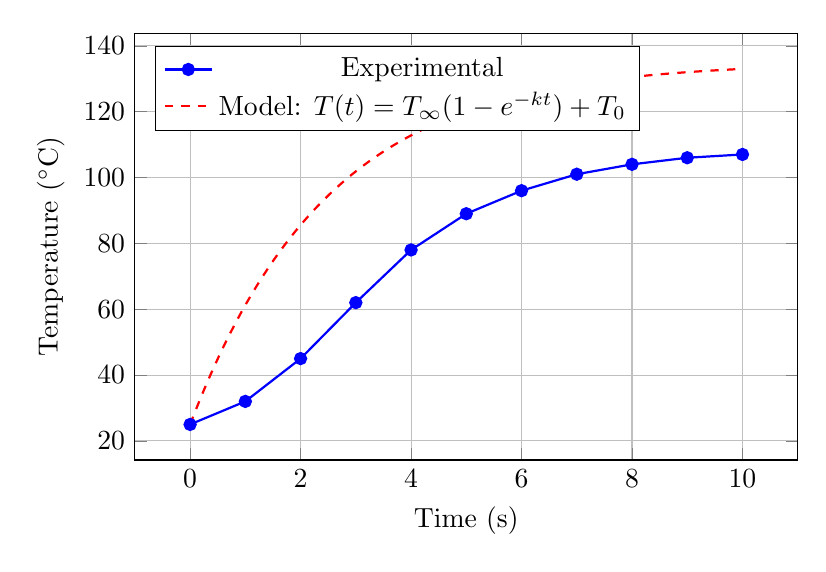
\begin{tikzpicture}
    \begin{axis}[
        width=10cm,
        height=7cm,
        xlabel={Time (s)},
        ylabel={Temperature ($^\circ$C)},
        grid=major,
        legend pos=north west,
        ylabel near ticks,
        xlabel near ticks
    ]
    
    % Sample data - exponential heating curve
    \addplot[blue, thick, mark=*, mark size=2pt] coordinates {
        (0, 25) (1, 32) (2, 45) (3, 62) (4, 78) 
        (5, 89) (6, 96) (7, 101) (8, 104) (9, 106) (10, 107)
    };
    \addlegendentry{Experimental}
    
    % Theoretical curve
    \addplot[red, thick, dashed, domain=0:10, samples=100] 
        {110*(1-exp(-0.4*x)) + 25};
    \addlegendentry{Model: $T(t) = T_{\infty}(1-e^{-kt}) + T_0$}
    
    \end{axis}
\end{tikzpicture}
\end{document}"

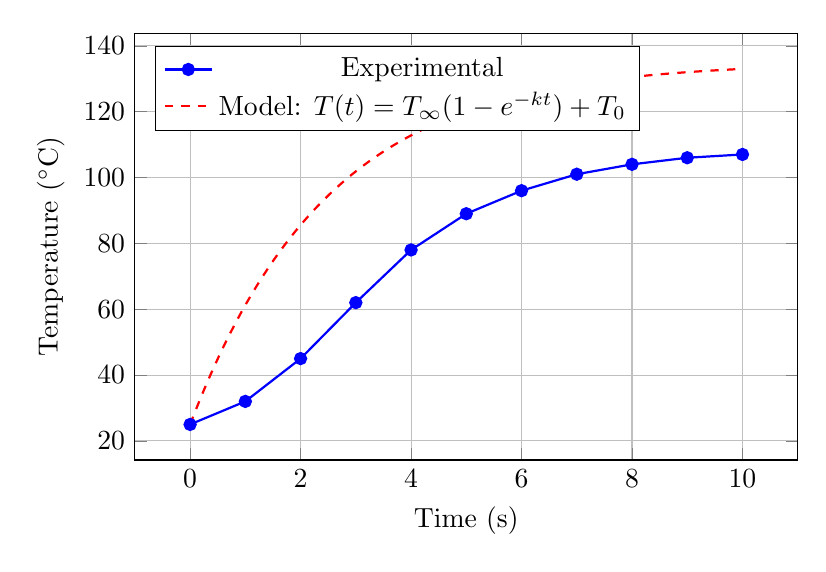
\begin{tikzpicture}
    \begin{axis}[
        width=10cm,
        height=7cm,
        xlabel={Time (s)},
        ylabel={Temperature ($^\circ$C)},
        grid=major,
        legend pos=north west,
        ylabel near ticks,
        xlabel near ticks
    ]
    
    % Sample data - exponential heating curve
    \addplot[blue, thick, mark=*, mark size=2pt] coordinates {
        (0, 25) (1, 32) (2, 45) (3, 62) (4, 78) 
        (5, 89) (6, 96) (7, 101) (8, 104) (9, 106) (10, 107)
    };
    \addlegendentry{Experimental}
    
    % Theoretical curve
    \addplot[red, thick, dashed, domain=0:10, samples=100] 
        {110*(1-exp(-0.4*x)) + 25};
    \addlegendentry{Model: $T(t) = T_{\infty}(1-e^{-kt}) + T_0$}
    
    \end{axis}
\end{tikzpicture}
